\documentclass[]{article}

\usepackage{amsmath}
\usepackage[]{graphicx}
\usepackage{subfigure}
\usepackage[latin1]{inputenc}
\usepackage{comment}
\usepackage{url}
%\usepackage{biblatex} 
%\usepackage[pdftex]{graphicx}
\usepackage{color}
\usepackage{anysize}
\marginsize{3cm}{3cm}{2cm}{2.5cm}%l r t b

\title{Using an Open Source Face Tracker for Identity Detection and Facial
Expression Recognition}
%\title{Controlling a smart phone using gaze gestures}
%\title{Gaze gestures as an innovative HCI method for smartphone like devices}
 
\author{Eduardo Neiva\footnote{Scholar at CNPq, National
Council for Scientific and Technological Development - Brazil}, Jesus Nuevo, David Rozado}

\setlength\parindent{0pt} %no indentation in paragraphs
% Document starts
\begin{document}

\maketitle

\section{Abstract}

Face and eye tracking technology are fairly well developed and robust technologies. Eye tracking in combination with
gaze estimation permits the monitoring of the user's area of attention on a computer screen while also providing a hint
about possible intention. Facial tracking can augment eye tracking by monitoring facial features that can convey the
identity of the user or its internal cognitive state as expressed through its facial expression. In this work, we use an
open source face tracker based on constrained local models and test its ability to classify a non-standard and broad
range of facial expressions and identities from continuous video input. Our results show that the face tracker is a
powerful tool to recognize the identity of a user among a large pool of subjects. We also show that our system can
robustly recognize facial expressions of users on which the system has been trained while also performing well on
recognising facial expression of faces not previously seen by the system. These positive results and the open source
nature of the system suggest the advantages and feasibility of augmenting traditional eye trackers by combining them
with face tracking algorithms as the one suggested here to enrich the set of features available to monitor a human while
interacting with a computer.


\section{Introduction}
Traditional Human Computer Interaction (HCI) could be augmented by providing computer systems with the ability to
recognize the emotions of the humans interfacing them. Emotions are conveyed by humans using visual, vocal
and other physiological means such as body gestures. Facial expressions are an indirect proxy to measure the internal
cognitive emotions of humans. Impaired facial expression recognition by humans can be a sign of serious cognitive
dysfunction such as schizophrenia \cite{Edwards2002789}.  Facial attributes can be tracked computationally through a
video stream of the subject's face. Making the computer aware of the emotions of the user could lead the way towards
more natural and fluid forms of interaction.


In this work we describe the usage of an open-source face tracker that feeds a set of machine learning classifiers
striving to identify subjects identity and their facial expressions. The face tracker provides a set of pose-invariant
deformation parameters estimated from the images. We use support vector machines (SVM) to classify the invariant
features provided by the face tracker.


The psychological literature has traditionally classified facial expressions in six categories, in addition to the
neutral expression: anger, disgust, joy, sadness and surprise~\cite{schmidt2002human}. In this work, we
also classify some additional facial gestures such as: raising eyebrows, open mouth, kissing face, closed smile and
squint face.


Researchers have employed a variety of methods to carry out facial expression recognition such as optical flow
computation  and symbolic representations \cite{Yacoob506414}, local binary patterns \cite{Shan2009803},  Bayesian
network classifiers \cite{Cohen1211408}, geometric deformation features and support vector machines
\cite{kotsia4032815}, hidden Markov models \cite{aleksic1597130, Cohen2003160}, Parametric flow models
\cite{blackAndYacoob}, AdaBoost and linear discriminant analysis \cite{bartlett1398364}. The surveys from
\cite{bartlett1398364} and \cite{Fasel2003259} are two good review sources about machine learning methods 
for fully automatic recognition of facial expressions. 


Previous work has employed a variety of techniques to classify  facial expressions. The work from \cite{Cohen2003160}
tested the classic neural network classifiers for classifying expression from video, focusing on changes in distribution
assumptions and feature dependency structures. The same authors also proposed and tested Hidden Markov Models (HMM) for
automatically segmenting and recognizing human facial expressions. Authors reported recognition rates up to 83\% for
frame-based recognition methods and 82\% for the multilevel HMM.


Chen et al.~\cite{Chen670976} investigated the emotional contents of speech and video based facial expression to
propose a bioinspired algorithm for human facial expression recognition, concluding that both modalities can be
complimentary and able to achieve higher recognition rates than either modality alone. Busso et al.~\cite{Busso:2004} also
used a multimodal approach to combine acoustic information and facial expression analysis in order to detect human
emotions. In their work, authors demonstrated that when both modalities are fused, the performance and the robustness of
the emotion recognition system improves considerably.


Bartlett et al.~\cite{Bartlett4624313} used perceptual primitives to code seven facial expressions in real-time. Their system
first detects frontal faces using a cascade of feature detectors trained with boosting techniques. The expression
recognizer receives image patches located by the phase detector. A Gabor representation of the parts is used  by a bank
of kernel based classifiers. Authors used a combination of Adaboost and support vector machines to enhance performance.
One of the most interesting properties of this work was its ability to change the outputs of the classifiers smoothly
as a function of time, hence, providing a dynamical representation of facial expression.

Databases available to the research community that include expression labeling have appeared in the last decade, of
which the Cohn-Kanade database~\cite{Cohn840611} is the best known. It contains over 2000 digitized image sequences from  182
adult subjects of varying ethnicity, performing multiple tokens of most primary facial expressions to create a
comprehensive testbed for comparative studies of facial expression analysis.


Facial identity recognition is another subject that has drawn a lot of attention in the research literature. While being
apparently trivial for humans to solve, automatic approaches have traditionally lagged behind the performance of humans
by at least one order of magnitude in terms of recognition performance. These approaches have only recently started to
catch up with the ability of the human brain to recognize faces \cite{onintelligence, Rozado2012b}. Face recognition is
important  for a wide range of commercial and law enforcement applications. Only recently has the technology required to
carry out automatic classification of faces become available. But the recognition of faces in outdoor environments 
where variation in pose and illumination are continuous remains a largely unsolved problem.


Zhao et al.~\cite{Zhao:2003} provide a good literature survey on the subject of face recognition. In
\cite{Craw1987183}, authors undertake an in-depth discussion of face features automatic extraction for classification
purposes of grayscale images. The work from \cite{Zhang20092876} undertakes a comprehensive review  of the challenging
topic of pose invariant face recognition, and while showing that the performance of different methods is still far from
perfect, several promising directions for future research  are suggested. Authors in \cite{Tan20061725} review the also
challenging topic of face recognition using  just one image per class for training and comparing several prominent
algorithms for the tasks. The rationale for the study is the reported critique that several face recognition techniques
rely heavily on the number of instances representative of each class on the training set.


In summary, in this paper we apply the open source face tracker described in \cite{saragih2011deformable} for identity
recognition and for facial expression recognition. We suggest that facial tracking can be a powerful complement to
traditional eye tracking  by augmenting the set of features being tracked during human computer interaction. This  can
potentially allow computer systems to more precisely monitor the cognitive state of the human interfacing them through
the proxy features of facial dynamics.


\section{Methodology}


\subsection{Face Tracker}
The face tracker used in this work is the regularised landmark mean-shift of Saragih et
al.~\cite{saragih2011deformable}\footnote{Source code is available at
  \url{https://github.com/kylemcdonald/FaceTracker}} an extension of
the original Constrained Local Model (CLM) of Cootes et al.~\cite{cristinacce2006feature}. We only present these methods
here briefly, and refer the interested reader to the original articles. CLMs try to fit a trained model to an unseen
face using a set of local classifiers to detect points of interest independently, and using a global point distribution model (PDM),
also referred as the \textit{shape model} to constrain the relative position of the points. Figure~\ref{fig:CLM}
illustrates the fitting process of CLM.

\begin{figure}[htbp]
  \centering
  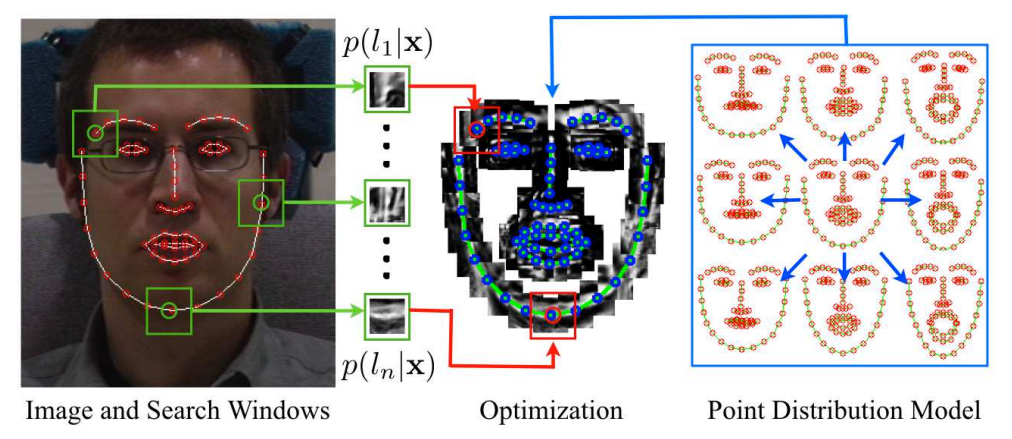
\includegraphics[width=0.95\textwidth,height=60mm]{figures/CLM.png}
  \caption{\textbf{Contrained Local Model Fitting}. The local patch classifiers generate surface responses, which are
  optimised together with the shape constraints. Courtesy of authors of~\cite{saragih2011deformable}.}
  \label{fig:CLM}
\end{figure}

The shape model is created from a training set. Non-rigid expressions are independent of the similarity transformation
of the face (scale, rotation and translation), so the shapes are transformed to a common reference frame and aligned,
typically using Procrustes method. From this set, the shape model is obtained using a dimensionality reduction technique
such as Principal Component Analysis (PCA). A new shape can then be generated as


\begin{equation}
  \label{eq:shape_model}
  \mathbf{x} = s\mathbf{R}(\bar{\mathbf{x}} +
  \boldsymbol{\Phi}\mathbf{q}) + \mathbf{t},
\end{equation}
were $\mathbf{x}$ is a vector with the landmark coordinates concatenated, 
$\{s,\mathbf{R},\mathbf{t}\}$ are the similarity transformation
parameters and $\mathbf{q}$ are the shape deformation parameters. The
shape model is defined by the \textit{mean shape} $\mathbf{\bar{x}}$
and the vectors of deformations $\boldsymbol{\Phi}$.


Patch classifiers are also created from a training set. In~\cite{saragih2011deformable} the classifiers are linear SVMs,
which makes computation of the surface responses very fast. The surface responses are composed with a sigmoid function,
which output can be treated as a probability map of the location of the landmarks. This location of each landmark in its
corresponding map is then optimised with constrained mean-shift, where the locations are updated using mean-shift
independent of each other, and are then constrained together by the shape model described above.


\subsection{Support Vector Machines}
Support vector machines (SVMs) have become popular as an efficient supervised learning model for automatic
classification. SVMs work by generating a set of hyperplanes that separate the training samples from different classes.
SVM achieve good generalisation by maximizing in training the distances between the hyperplanes and the nearest
data points of the different classes. Whenever the classification problem is not linearly separable in the
space of the data samples, kernel functions may be used to map the original feature space into a much
higher-dimensional space in order to achieve linear separation.

Since SVMs make a binary decision, a multi-class one-to-one classification approach was used for dealing with the
several classes (facial shapes) involved in our experiments. This work has used the open source SVM library
LIBSVM\footnote{\url{http://www.csie.ntu.edu.tw/~cjlin/libsvm/}}. The library is available in many languages and
supports most of the functionality associated to SVM classification.


\subsection{Experimental Setup}
The dataset that was used to train and test the classification algorithms was specifically generated for this work. We
generated the data set of facial expressions from scratch instead of using existing data sets of facial expressions in
order to gain freedom in terms of the number of facial shapes available for testing. This was due to our objective of
analyzing our system under challenging conditions beyond the classical six or seven facial expressions usually employed
on the literature about automated facial expression  recognition. Hence, we recorded 11 facial shapes or facial
expressions. In this work, we employ the terms facial shape or facial expression interchangeably. The data set consists
of 50 people (age distribution ranged from 19 to 40 years old). From the entire set, 80\% were male and 20\% female. In
terms of ethnicity, 16\% were Latino, 10\% were Asian and the rest were Caucasian. The data capture was made using a
standard notebook webcam, 1.3 MP, running at a resolution of 640x480. The distance between the camera and the subject's
face was about 114cm. The data extracted from the face tracker was a vector with 24 dimensions that represents a
particular face shape at any given time point. This vector has the property of being invariant to changes in scale,
rotation and translation but provides a distinguishing signature for different facial expressions and facial identities.


\subsubsection{Methodology of the data capture}
Every participant involved in the experiment was asked to perform eleven different facial shapes or expressions
\ref{dataExtrationExamples}. Six of them were stereotypical emotions common to every person: neutral, anger, disgust,
joy, sadness and surprise. The remaining facial expressions where: open mouth, raised eyebrows, kissing face, closed
smile and squint face. Even though the feature vector produced  by the face tracker was invariant to changes in scale,
the distance between the camera and the subject was kept constant to maintain uniformity conditions among subjects
during the data collection.


\begin{figure}[ht]
\begin{center}
\vspace{-3mm}
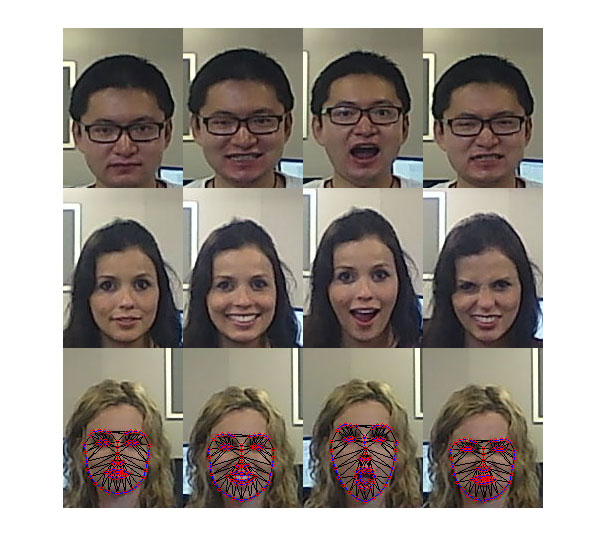
\includegraphics[width=0.95\textwidth,height=90mm]{figures/dataExtrationExamples.jpg}
\end{center}
\caption{\textbf{Data Gathering}. Fifty subjects overall were recruited and asked to perform 11 types of facial shapes during a 
recording session. We strove to  get a diverse representation of gender, ethnicity and age. The bottom row shows the facial tracker 
model superimposed over one of the subjects participating in the experiment.}
\label{dataExtrationExamples}
\end{figure}


Each participant was given a chance to familiarize with the system and to try out all the different facial expressions
to pose during the data capture phase. After this familiarization stage with the system, the subject was told to perform
again the 11 face shapes, this time for recording purposes. For every face shape category, 20 samples were recorded with
a small time interval between them (less than one second). Each sample consisted on capturing the invariant vector
provided by the eye tracker that transforms a neutral face shape into the deformed face shape that fits the subject
facial expression. Since often there were fluctuations on the borders of the face being tracked and this generated some
instability on the invariant vector, 20 samples were taken to smooth out this noise. This data was subsequently
used for training and validation. We used the entire 24 features of each face shape. 


During the data capturing period, we observed that every person had a unique invariant vector signature associated to
each facial expression. These signature vectors were also highly correlated across subjects but not quite identical.
Hence, we decided to test how this invariant feature vector could be used to recognize facial identity as well as facial
expressions. The invariant feature vector specific for each person and facial expression contains an invariant
representation of the dots that conform the grid seen in the last row of Figure
\ref{comparationBetweenFaces}. Thus the goal of the SVMs task was two-fold: to generate an abstraction of each facial
expression class in order to be able to carry out facial expression classification, and to be able to cluster facial
expressions of different people across identities in order to carry out facial identity recognition.


\subsubsection{Experiment}\label{experimentsSubsection}
The first experiment tried to recognize people's identity using the entire data set of the study participants. The
training and test set data were generated by splitting 70\% of the samples of each person and using it to train the SVM
and using the remaining 30\% for testing. 10-fold cross validation was applied for all the conditions during the
validation procedure. Three different training conditions were used for this experiment. For all the training conditions, the
experiment was conducted by increasing the number of people in the experiment and testing the resulting accuracy. The 3
training conditions analyzed were:

\begin{description}
	\item[$\bullet$ Only Neutral Face:] Only the neutral face shape was used in this
	experiment.   
	\item[$\bullet$ Six Face Shapes:] Six face shapes were used in this experiment (neutral,
	opened mouth, smiling, raised eyebrow, surprise and anger face). All of those
	shapes were clustered into a unique class associated to each
	participant. 
	\item[$\bullet$ Eleven Face Shapes:] All the face shapes (11) were used in this condition. All of those
	shapes were clustered into a unique class associated to each participant. 
\end{description}

For the face shape recognition experiment, there were two different methods of training that were used throughout the
experiments. All of them used a 7:3 ratio for training and testing respectively. 10-fold cross validation was
applied in all experimental conditions during the validation procedure. The procedure is conducted
by increasing step by step the number of people in the experiment and testing the resulting
accuracy. The 2 training conditions analyzed were:

\begin{description}
	\item[$\bullet$ Including:] The training and test set shared the same group of participants. Only different instances
	of each facial expressions were used for the training and test sets. By different instances of a face shape we mean
	that the face shape instances were captured at different time slots. The entire 11 face shapes classes were used in
	this experiment.
	\item[$\bullet$ Excluding:] The training and test set did not share the same group of participants. That is, the faces
	in the test set corresponded to subjects not included in the training set (disjoint across facial identity). The entire
	11 face shapes classes were used in this experiment.
\end{description}


In order to study how increasing the number of face shapes to recognize degrades performance, we designed a third
experiment. Its goal was to analyze the impact on accuracy of increasing the number of face shapes (classes).  In this
experiment, the training and test sets were disjoint across facial identity (did not share the same subjects).
The data set was partitioned in 70\% for training and 30\% for testing. The experiment was carried out by increasing the
number of face shapes (classes) in the experiment and testing the resulting accuracy.

\begin{figure}[ht]
\begin{center}
\vspace{-3mm}
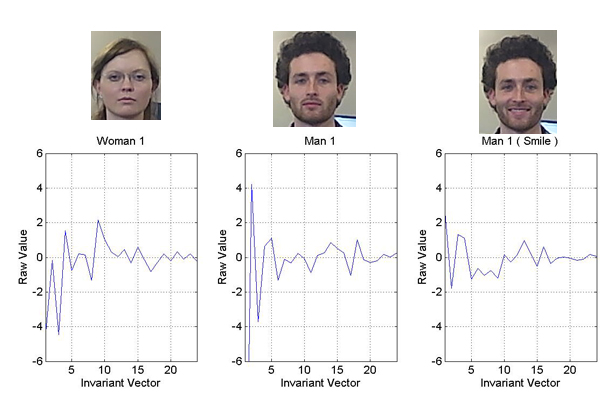
\includegraphics[width=0.95\textwidth,height=75mm]{figures/comparationBetweenFaces2.jpg}
\end{center}
\caption{\textbf{Invariant and Unique Feature Vectors of Facial Expressions.} This figure displays typical feature 
vector signatures specific for a given person. The characteristic feature vector can be used to recognize people. The
feature vector provided by the face tracker changes for each facial expression performed but remains invariant within a
given facial expression. Furthermore, features vectors of the same facial expression among different people share commonalities that
can be exploited to carry out facial expression recognition among different people.}
\label{comparationBetweenFaces}
\end{figure}

A video demonstration sample of the signature vector changes across people and facial expressions is available at:
\url{ http://youtu.be/zhocLU5NXDU}

\section{Results}

\subsection{Recognizing Facial Identity}
We tested first the ability of our classification algorithms to detect facial identity. In these set of experiments,
each person to be recognized represents a class. Therefore, increasing the number of people in the data set to recognize
increases the number of the classes and the difficulty for the classification algorithm. We tested the performance of
the algorithm on the range of 2 to 50 people and under three different conditions: facial identity classification based
on only the neutral face, facial identity classification based on 6 face shapes and facial identity classification based
on 11 face shapes. The specifics of each of these experimental conditions are described in Subsection
\ref{experimentsSubsection}.


It is expected that as we increase the number of people in the experiment, accuracy would be reduced due to the growth
of classes in the problem. It is also expected  that using less face shapes to model one person reduces the complexity
of the classification model and thus this results in higher accuracy performance. Figure \ref{identityRecognition},
shows that to recognize 50 people using only neutral faces resulted in 98.1\% recognition accuracy.  When using 6 face
shapes, accuracy decreases to 82.9\% and using 11 face shapes accuracy decreases it further to 76.02\%.


\begin{figure}[ht]
\begin{center}
\vspace{-3mm}
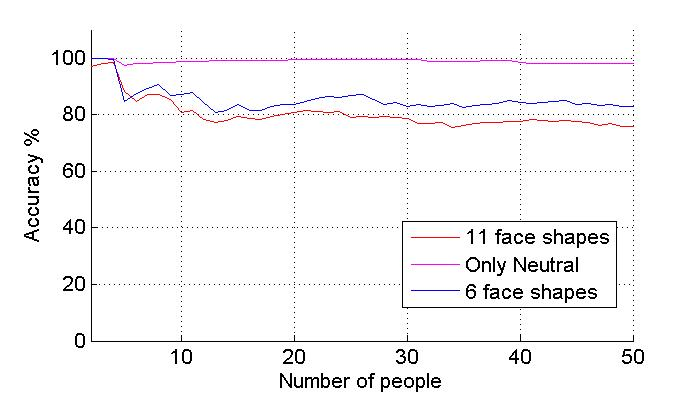
\includegraphics[width=0.95\textwidth]{figures/peopleRecognition4.jpg}
\end{center}
\caption{\textbf{Facial Identity Recognition Results.} The face tracker engine used in this work can be employed 
to recognize the identity of the face since the feature vector generated by the face tracker is characteristic for
different faces. Facial identity recognition performed very well when using the training set consisting exclusively
of neutral faces. Performance degraded slightly as we increased the number of facial shapes in the training set, 
but still the system shows robust  recognition performance.}
\label{identityRecognition}
\end{figure}


\subsection{Recognizing Face Shapes}
In this experiment, the goal was to recognize each of the 11 different classes of facial expressions or face shapes in
the training set. We measured two different experimental conditions. These different experimental conditions are
described in Subsection \ref{experimentsSubsection} and we refer to them as ``Including'' and ``Excluding''. For the
first method ``Including'', the subjects included in the training set were the same as the subjects included on the test
set. The sets only differ by the instances present in each of them (feature vectors captured at different time points).
This facilitated considerably the classification task and we expected to obtain high classification accuracy. For the
``Excluding'' experimental condition, the subjects in the training and test sets were disjoint. That is, the
classification algorithm was tested on facial identities to which it had not been exposed to during training. For this
experimental condition, we expected worse performance than in the ``Including" condition but a gradual improvement in
performance as more face shapes added to the training set cover a wider range of possible facial shapes configuration.
This improvement was expected up to a point from which on, the system would start to gradually decrease in performance
by reaching the saturating capacity of the classification model. However we never reached a saturation point with our
data set as evidence by Figure \ref{feRecognition}. The accuracy obtained with 50 participants using the ``Excluding''
experimental condition was 57.18\%, and 90.5\% when using the ``Including'' experimental condition.
 
<<<<<<< HEAD
 
After completing the experiment, a standard way to analyze the behavior of each class during a classification task is by
creation of a confusion matrix. This permits the visualization of the most problematic classes. Since the classification
task was to predict face shapes, some facial expressions were expected to have considerable overlapping error due the
facial shapes being similar, the Figure \ref{coExcluding} shows that from the ``Excluding'' methodology, we have this
effect on some face shapes, such as the squint face shape, for which in 17\% of its cases is predicted as being a
neutral face and the raised eyebrow face shape being predicted as neutral 10.15\% of the cases.
On the Table \ref{rankEx} it is seen how often each face shape returns
true positives. Similar effects can be observed in the better performance ``Including'' experimental condition in Figure
\ref{coIncluding} and in Table \ref{rankIn}. 


\begin{figure}[ht]
\begin{center}
\vspace{-3mm}
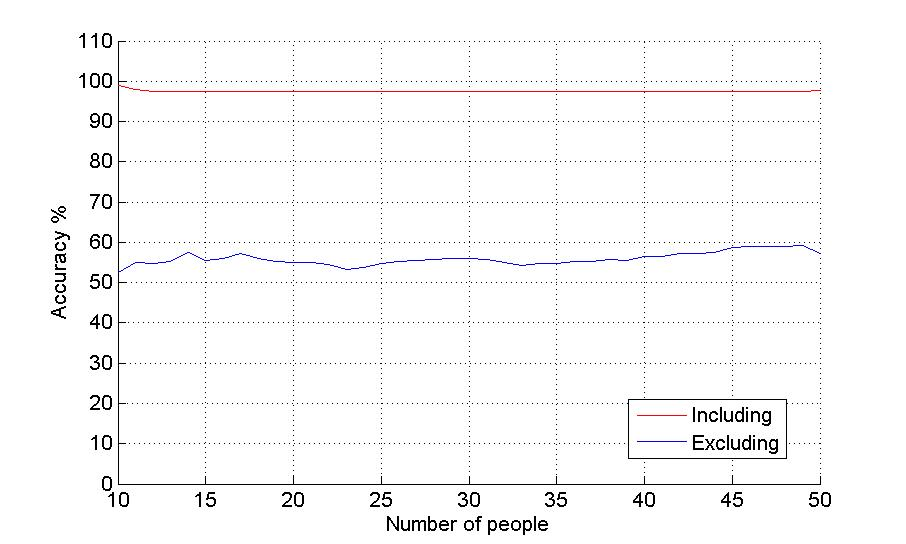
\includegraphics[width=0.95\textwidth]{figures/figureRecognizeFacialExpressionTrue.jpg}
\end{center}
\caption{\textbf{Facial Expression Recognition Results.} This figure shows the result of the facial expression
recognition experiment. The curve labeled ``Including'' partitions the data set into training and test sets, but that
training and test sets belong to the same participants. The curve labeled ``Excluding'' represents the much harder
problem of recognizing facial expressions of unknown subjects (subjects not included in the training phase). Still, the performance 
of the system was quite robust as the number of people increased and never saturated to the point of starting to
degrade in terms of performance.}
\label{feRecognition}
\end{figure}


\begin{figure}[ht]
\begin{center}
\vspace{-3mm}
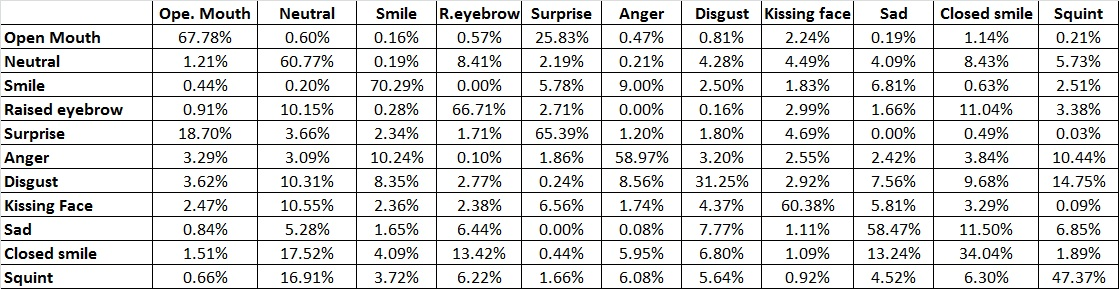
\includegraphics[width=0.95\textwidth]{figures/confusionExcluding.jpg}
\end{center}
\caption{\textbf{Confusion Matrix for the ``Excluding'' Experimental Condition.} This figure
shows the confusion matrix for the excluding experimental condition. The left column represents the
actual class that should be recognized whereas the upper row represents the
predicted class. In this table, it is seem, for example, that due the similarity
of the Open mouth and Surprise face shape, 25 percent the Open mouth instances were
incorrectly classified.}
\label{coExcluding}
\end{figure}

\begin{table}[t]
\centering
\begin{tabular}{|l|c|}
\hline
Face Shapes & Accuracy(\%) \\ \hline
Smile & 70.2\\ \hline
Open Mouth & 67.7\\\hline
Raised eyebrow & 66.7\\\hline
Surprise & 65.3\\\hline
Neutral & 60.7\\\hline
Kissing Face & 60.3\\\hline
Anger & 58.9\\\hline
Sad & 58.4\\\hline
Squint & 47.3\\\hline
Closed Smile & 34.0\\\hline
Disgust & 31.2\\\hline
\end{tabular}
\caption{\textbf{Individual Results for Classification for the 'Excluding'
Experimental Condition.} This table shows the effectiveness of the algorithm over each individual face
shape. The face shape smile, open mouth and raised eyebrow showed to be predicted most accurately.}
\label{rankEx}
\end{table}




\begin{figure}[ht]
\begin{center}
\vspace{-3mm}
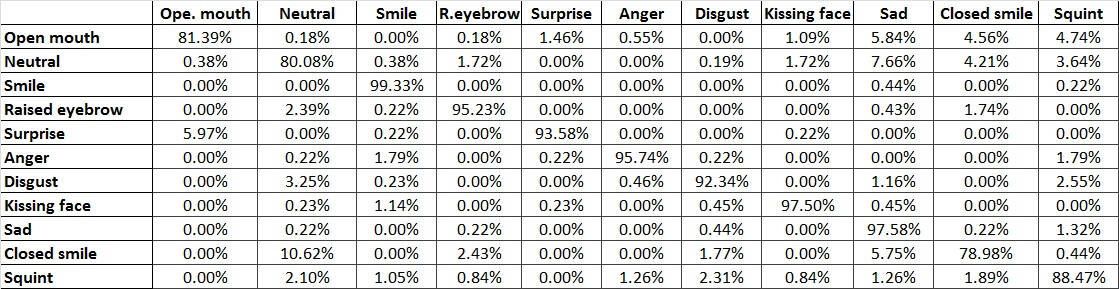
\includegraphics[width=0.95\textwidth]{figures/confusionIncluding.jpg}
\end{center}
\caption{\textbf{Confusion Matrix for the ``Including'' Method.} This figure 
shows the confusion matrix for the including method. The left column represents 
the actual class that should be recognized whereas the upper row represents the 
predicted class. In this table, it is obvious the better performance of this experimental condition over the
``Excluding" condition. Still some of the same effects observed in the ``Including" confussion matrix in terms of
facial shapes commonly misclassified as being a different class are still present.}
\label{coIncluding}
\end{figure}

\begin{table}[t]
\centering
\begin{tabular}{|l|c|}
\hline
Face Shapes & Accuracy(\%) \\ \hline
Smile & 99.3\\\hline
Sad & 97.5\\\hline
Kissing face & 97.5\\\hline
Anger & 95.7\\\hline
Raised & 95.2\\\hline
Surprise & 93.5\\\hline
Disgust & 92.3\\\hline
Squint & 88.4\\\hline
Open mouth & 81.3\\\hline
Neutral & 80.0\\\hline
Closed smile & 78.9\\\hline
\end{tabular}
\caption{\textbf{Indivudal Results for Classification for the ``Including''
Method.} This table shows the effectiveness of the algorithm over each individual face
shape. The face shape smile, sad and kissing face showed to be predicted most accurately.}
\label{rankIn}
\end{table}

 
\subsection{Recognizing Face Expressions results by changing the number of classes}
The last experiment looked at how increasing the number of face shapes to recognize impacts performance. Figure
\ref{increasingNumberExpressions} shows the results of increasing the number of face shapes to be recognized by the
classifier. In this experiment, the goal was to evaluate the impact on accuracy of increasing  the number of classes to
be recognized. The methodology described at the end of Subsection \ref{experimentsSubsection} was used in this
experiment. It was expected that the algorithm would gradually decrease in accuracy efficiency as we included more
facial shapes (classes). The accuracy for 4 classes was 95.1\% and for 7 classes was 73.2\%.


\begin{figure}[ht]
\begin{center}
\vspace{-3mm}
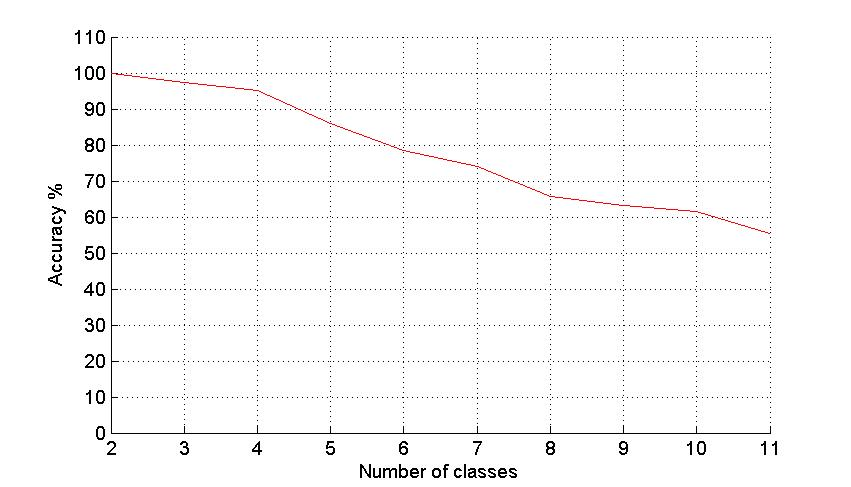
\includegraphics[width=0.95\textwidth]{figures/50people_increasing_classes.jpg}
\end{center}
\caption{\textbf{Effect of Increasing the Number of Facial Expressions to Recognize.} This figure displays how the 
performance of the system degrades as the number of classes or face shapes to recognize is increased. }
\label{increasingNumberExpressions}
\end{figure}






\section{Discussion}
In this work we have used an open-source face tracker based on regularised landmark mean-shift to recognize facial
identity and to classify facial expressions. The face tracker provided a feature vector invariant to scale, rotation and
translation transformations. A person adopting a given facial shape would generate on the face tracker an invariant
feature vector that we called through the paper signature vector. This signature vector would change with each facial
expression  and among different subjects. Still, the similarities among people adopting the same facial expression 
allowed for facial expression recognition of subjects unexposed to the system during training.


The proposed system shows an extremely strong performance for recognizing facial expressions of persons whose facial
expressions were used to train the system (close to 100\%). Performance degrades considerably when using the system to
recognize facial expressions of subjects that were not used during the training phase. Still, this is an extremely
challenging problem, and the performance of the system is encouraging, robust and improving as the number of faces
in the training set increases.


Obviously the larger the amount of classes (facial expressions) to classify, the more challenging the
classification problem is. In this work, we did not limit ourselves to the traditional set  of six facial expressions
used in the literature on the subject. We have included additional facial expressions or more appropriately facial
shapes in order to test the performance of our approach in challenging environments. Obviously, the performance of the
proposed method degrades as the number of classes  or facial shapes increases, but the decrease is smooth with no abrupt
negative slopes as the number of facial shapes is increased over the different experimental trials.


When we observed the distinctive feature vectors signature associated to each individual face, we immediately thought
about the application of using the face tracker engine to recognize facial identity. The algorithm performed extremely
well  through the whole range of testing conditions that we tested (using only neutral faces, using six facial
shapes and using 11 facial shapes). The algorithm proved to be extremely robust to recognize the identity of face using
just a neutral face, with performance almost as high as 100\%.

The initial motivation for this work was to test a face tracker in the recognition of facial expressions in order to
augment existing gaze tracking systems. The fusion of face and gaze tracking modalities can provide additional
information about the internal cognitive state of the subject interfacing a computer system. We have shown that the data
provided by this open-source face tracker is enough on its own to generate a rich source of information that can be
used to monitor a user emotional status. The open source nature of the software makes its distribution and adoption by
the research community extremely easy. Also, the very basic hardware requirements required by the face tracker, just a normal web
camera, further facilitates its adoption and dispersion within the research community.


In summary, we have shown here how an open source face tracker using regularized landmark main shift can be successfully
used to recognize facial identity and facial expression. Future work should try to integrate the data provided by an
eye tracker with the data provided by the face tracker in order to show how the combination of both tracking modalities
augments and improves the monitoring capabilities of either system on its own.



\bibliographystyle{plain}
\bibliography{library,extrabib}

\end{document}
